\documentclass[10pt, t]{beamer}
% \usepackage[UTF8]{ctex}
\usepackage{amsmath}
\usepackage{setspace}
\usepackage{float} 
\usepackage{multido}
\usepackage{multirow}
\usepackage{array}
\usepackage{enumerate}
\usepackage{booktabs}
\usepackage{indentfirst} 
\usepackage[style=mla]{biblatex}
\usepackage{setspace}
\usepackage{subcaption}
\usepackage{hyperref}
\usepackage{textpos}
% \usepackage{fontspec}

% \beamerdefaultoverlayspecification{<+->}
\makeatletter
\let\@@magyar@captionfix\relax
\makeatother

\definecolor{bladerunnerblue}{RGB}{41, 159, 163}
\definecolor{bladerunnerred}{RGB}{194,84,97}
\definecolor{themecolor}{RGB}{25,25,112} 
\definecolor{weak}{RGB}{150,150,150}

\renewcommand{\emph}[1]{{\color{themecolor}\textsl{#1}}}
\newcommand{\alarm}[1]{{\color{bladerunnerred}{#1}}}
\newcommand{\N}{\mathbb{N}}
\newcommand{\R}{\mathbb{R}}
\newcommand{\dom}{\operatorname{dom}}
\newcommand{\myseries}[2]{$#1_1,#1_2,\dots,#1_#2$}
\newcommand{\nullspace}{~\\[15pt]}
\newcommand{\remark}{\textbf{Remark: }}
\newcommand{\question}{\textbf{Question: }}
\newcommand{\scp}[2]{\langle\,#1\,,\,#2\,\rangle} \newcommand{\scpp}{\langle\,\cdot\,,\,\cdot\,\rangle}
\newcommand{\weaken}[1]{{\color{weak}\textit{#1}}}
\newcommand{\underover}[3]{\underset{#2}{\overset{#3}{#1}}}
\renewcommand{\emptyset}{\varnothing}


\usetheme{Madrid}
\setbeamertemplate{navigation symbols}{}

\addtobeamertemplate{frametitle}{}{
\begin{textblock*}{100mm}(0.85\textwidth,-1cm)
\includegraphics[height=1cm]{../../logo.png}
\end{textblock*}}


\usecolortheme[named=themecolor]{structure}

\setbeamertemplate{items}[default]

\hypersetup{
    colorlinks=true,
    linkcolor=themecolor,
    filecolor=themecolor,      
    urlcolor=themecolor,
    citecolor=themecolor,
}

\title{VV186: Honors Mathematics}
\subtitle{Functions \& Differentiation}
\institute[UM-SJTU JI]{Univerity of Michigan-Shanghai Jiao Tong University Joint Institute}
\author{Xingjian Zhang}

\begin{document}

\begin{frame}
    \titlepage
    \begin{center}
        \includegraphics[height=2cm]{../../logo2.png}
    \end{center}
\end{frame}

\begin{frame}
    \frametitle{RC Policy}
    Several things I want you to pay attention to:
    \begin{enumerate}
        \item \alarm{Be interactive.} Feel free to interrupt me at any time if you want to ask something or simply make some comments. You are free to discuss with your friend if you want, as long as your discussion is related to the course contents and your voice won't effect other students.
        \item Speak everything in \alarm{English} during the RC. This might be hard at the beginning, but you will soon get used to that.
        \item \alarm{``Question everything.''} Do not pretend to have understood everything. Maths is about strictness, abstraction and generalization. Understanding every basic concept is essential in our course. I will be quite ``push'' on checking your conceptual understanding. This process will be \textbf{annoying, tedious, but rewarding}. So Get prepared.
    \end{enumerate}
\end{frame}

\begin{frame}
    \frametitle{Outline}
    \begin{spacing}{1}
        \tableofcontents
    \end{spacing}
\end{frame}

\section{Midterm 1}
\subsection{Distribution}
\begin{frame}
    \frametitle{About Midterm 1}

    \begin{figure}[H]
        \centering
        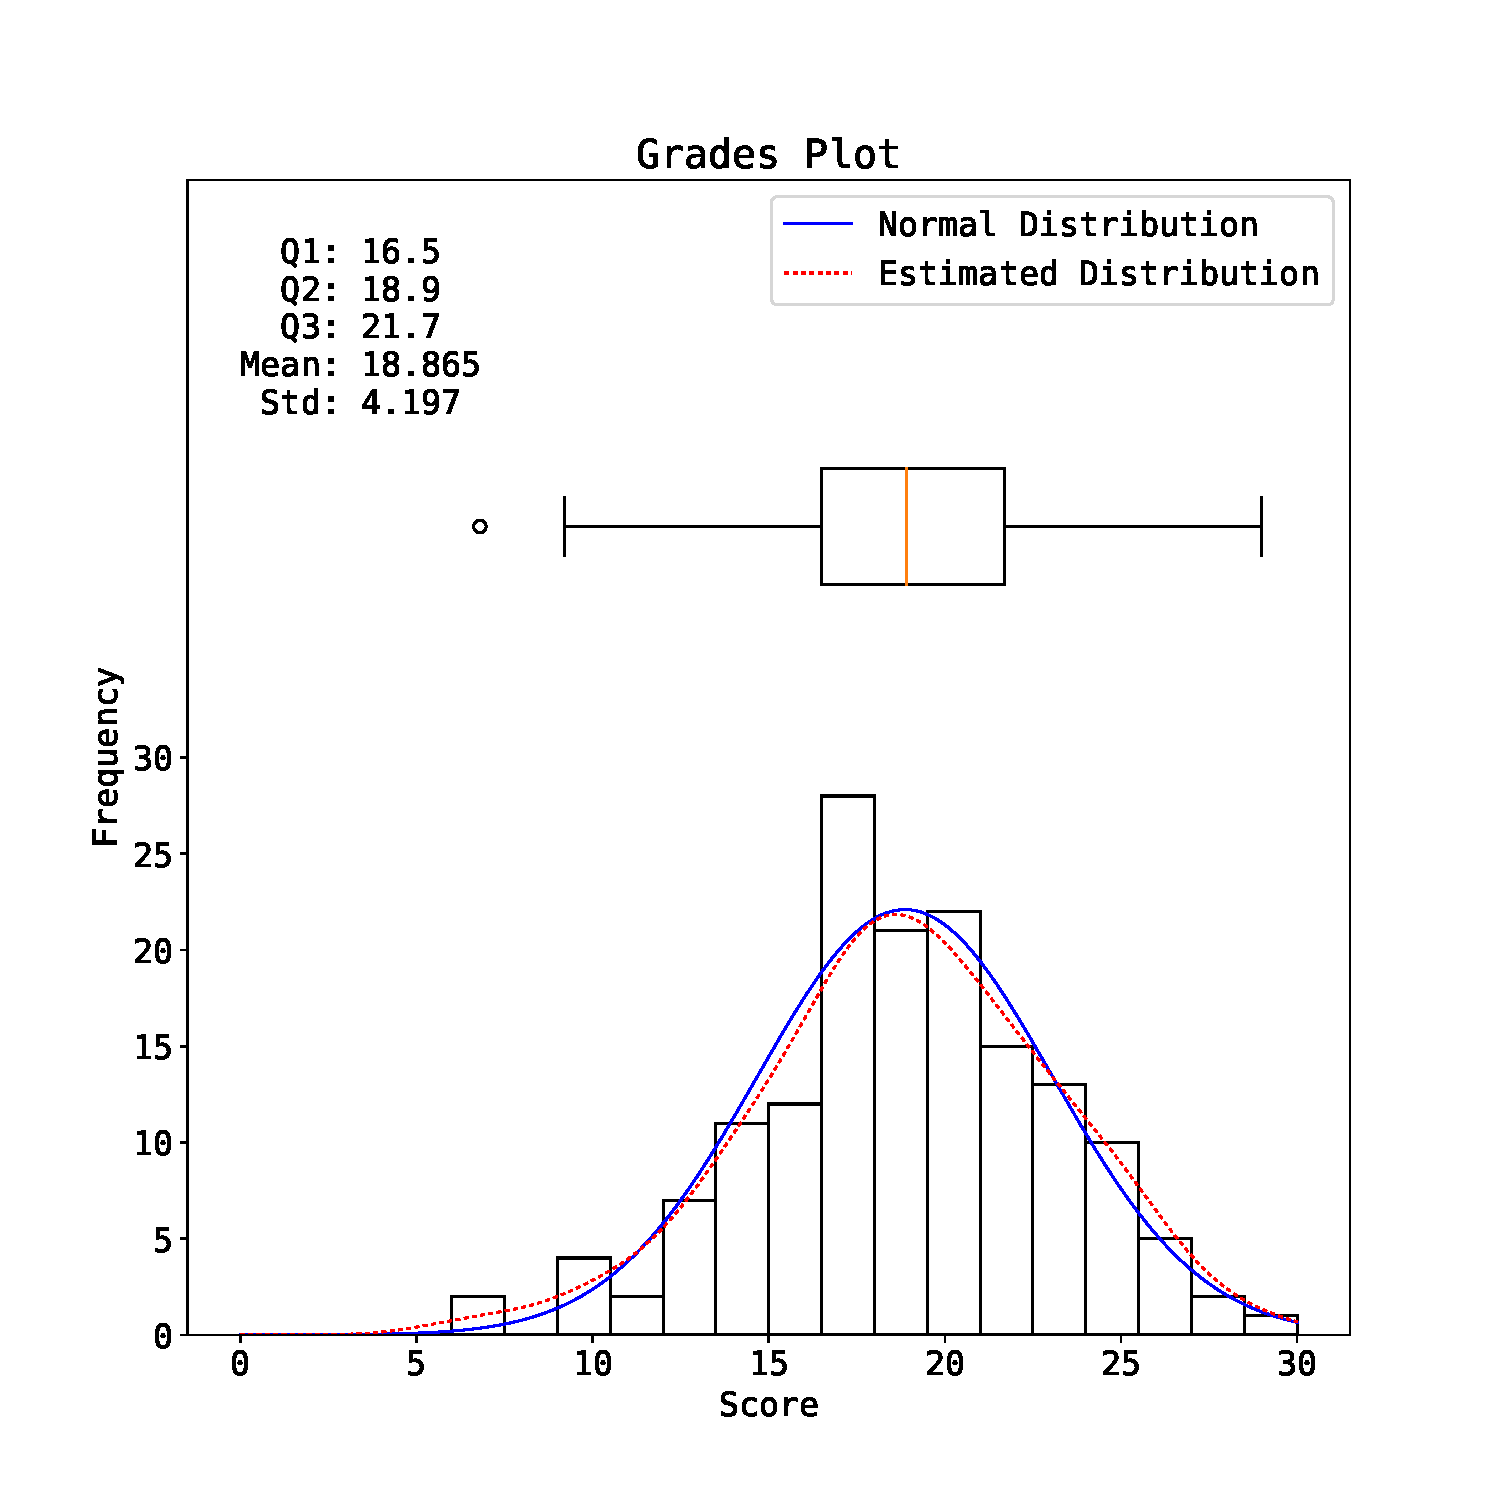
\includegraphics[width=0.6\textwidth]{./mid1dist.pdf}
    \end{figure}

\end{frame}

\subsection{Ex6}
\begin{frame}
    \frametitle{About Ex.6}
    For a continuous increasing function $f$,\footnote[frame]{Mean of Ex.6: 1.09'(4')}
    \begin{itemize}
        \item $\underset{x\to -\infty}{\lim}f=0$
        \item $\underset{x\to \infty}{\lim}f=\infty$
    \end{itemize}
    How to decompose the proof? (We have discussed this strategy in our first RC.)
    \begin{enumerate}
        \item Prove $\operatorname{ran} f\subset (0,\infty)$
        \item Prove $\operatorname{ran} f\supset (0,\infty)$
    \end{enumerate}
    How to prove 1.?
    \begin{itemize}
        \item Any $f(x_0)\leq 0$ leads to a contradiction.
        \item Use the definition of \emph{limit} and \emph{strictly increasing} to show how they contradict rather than simply stating a contradiction occurs.
    \end{itemize}
    How to prove 2.?
    \begin{itemize}
        \item $\forall y\in(0,\infty)\,\exists x\in \R :f(x)=y$
        \item Use the \emph{intermediate value theorem} and the definition of \emph{limit} to show how $x$ can be found.
    \end{itemize}
\end{frame}

\begin{frame}
    \frametitle{Comments}

    \begin{itemize}
        \item The exam is quite different from high school exam. Do not panic if you did not get a nearly full mark. Instead, compare with \emph{mean}, \emph{quartiles}.
        \item Take a deep breathe. Reflect why you did well in some exercises but bad in some others.
        \item Think like a mathematician, write like a mathematician. Especially in proof, you are expected to give a strict proof based on our strict definition of concepts. (I see many people consider $\infty$ as if it was a number.)
        \item If you feel it necessary for you to see what happens in grading for your exam paper. Go to Horst's exam inspection session. It will be announced recently.
        \item If you feel frustrated, definitely come to my OH so we can have a chat. That will help you figure out what you can do to improve.
    \end{itemize}
\end{frame}

\section{Differentiation}
\subsection{Leibniz Notation}
\begin{frame}
    \frametitle{Leibniz Notation}
    \emph{Leibniz Notation} is a powerful, versatile, flexible notation system for calculus (and even differential geometry, etc). We regard $dy$ and $dx$ as infinitesimal elements, therefore have a good intuition of them. We can then rewrite many useful formulas in Leibniz notation:
    \begin{itemize}
        \item Chain rule: $$\frac{d f}{d x}=\frac{d f}{d g} \cdot \frac{d g}{d x}$$
        \item Inverse function theorem: $$\frac{d x}{d y}=\frac{1}{\frac{d y}{d x}}$$
    \end{itemize}
    \textbf{Remark:}
    \begin{itemize}
        \item
              In the coming future, we will see its power in integral calculus, too.
        \item
              Despite its flexibility, keep in mind we still need to verify these formulas  like above using strict definition.
        \item
              You are free to use Leibniz notation in your coursework if you want.
    \end{itemize}
\end{frame}

\begin{frame}
    \frametitle{Exercise}

    We define the \emph{hyperbolic cosine} and \emph{hyperbolic sine} functions by
    $$\cosh , \sinh : \mathbb{R} \rightarrow \mathbb{R}, \quad \cosh x:=\frac{1}{2}\left(e^{x}+e^{-x}\right), \quad \sinh x:=\frac{1}{2}\left(e^{x}-e^{-x}\right)$$
    \begin{enumerate}
        \item
              Show that $\sinh : \mathbb{R} \rightarrow \mathbb{R}$ is bijective (and hence invertible). Verify that
              $$
                  (\sinh x)^{\prime}=\cosh x
              $$
              then express the derivative in terms of sinh.
        \item
              The inverse function of sinh is called the area hyperbolic sine, written Arsinh: $\mathbb{R} \rightarrow \mathbb{R}$. Use the inverse function theorem to prove that
              $$
                  (\operatorname{Arsinh} x)^{\prime}=\frac{1}{\sqrt{x^{2}+1}}
              $$
    \end{enumerate}
\end{frame}

\subsection{Extrema}
\begin{frame}
    \frametitle{Extrema}

    \begin{figure}[H]
        \centering
        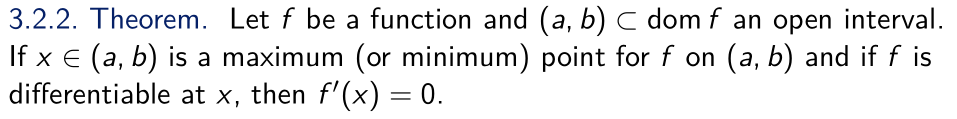
\includegraphics[width=0.9\textwidth]{2020-11-04-11-56-14.png}
    \end{figure}

    \textbf{Remark:} Notice the condition: why open interval?

    \begin{figure}[H]
        \centering
        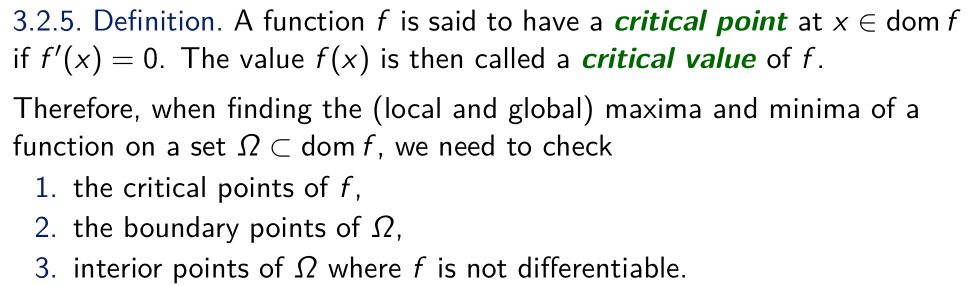
\includegraphics[width=0.9\textwidth]{2020-11-04-12-07-34.png}
    \end{figure}

\end{frame}

\begin{frame}
    \frametitle{Critical Points}

    \begin{figure}[H]
        \centering
        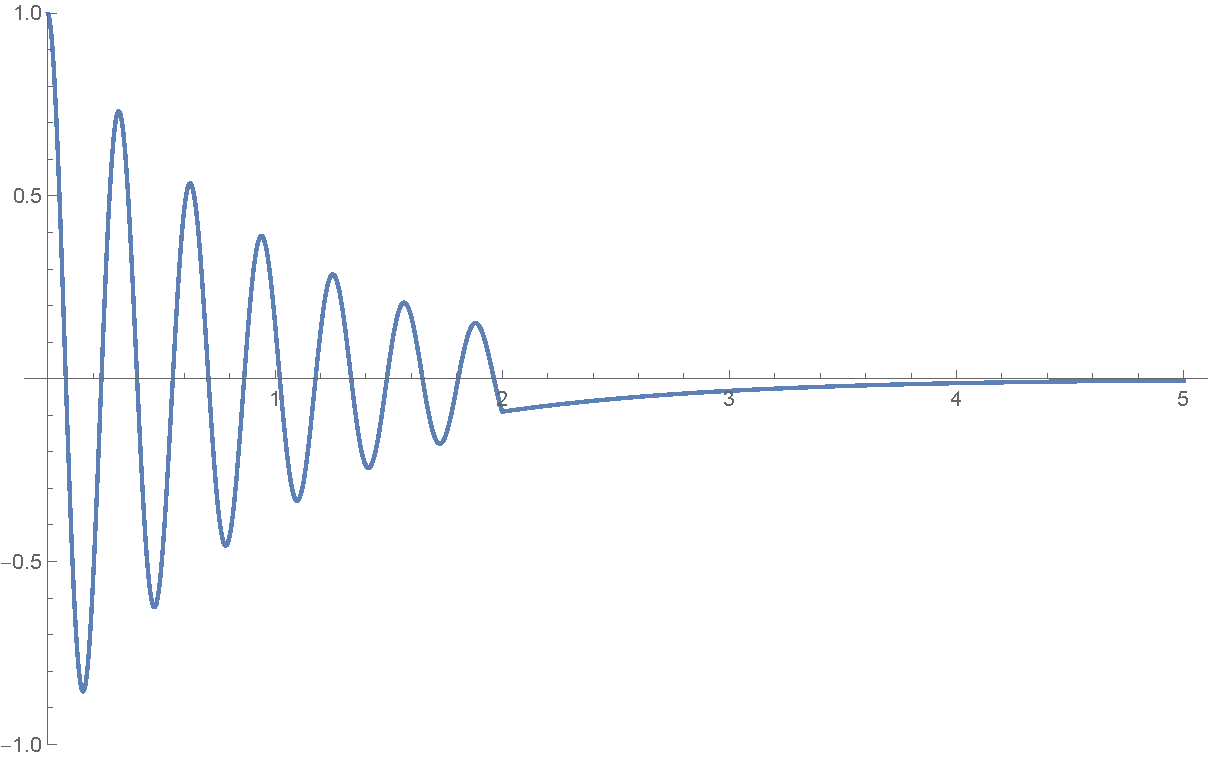
\includegraphics[width=0.6\textwidth]{extrema.pdf}
    \end{figure}
    Point out
    \begin{enumerate}
        \item global maxima
        \item global minima
        \item all local maxima
        \item all local minima
        \item critical points
        \item boundary points
        \item indifferentiable interior points
    \end{enumerate}
\end{frame}

\begin{frame}
    \frametitle{True or False?}

    If $f'(x)=0$, then $x$ is a local extrema point for $f$.

    \pause
    False, counter-example:
    \begin{figure}[H]
        \centering
        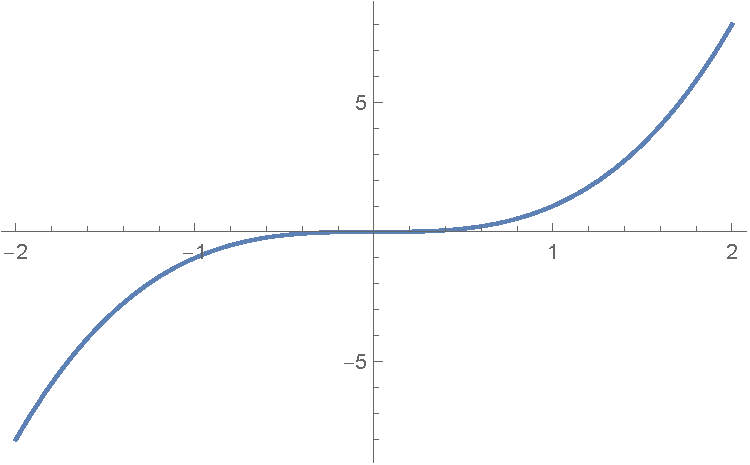
\includegraphics[width=0.6\textwidth]{extrema2.pdf}
        \caption{$f(x)=x^3$}
    \end{figure}
\end{frame}

\subsection{Mean Value Theorem}
\begin{frame}
    \frametitle{Mean Value Theorem}

    \begin{figure}[H]
        \centering
        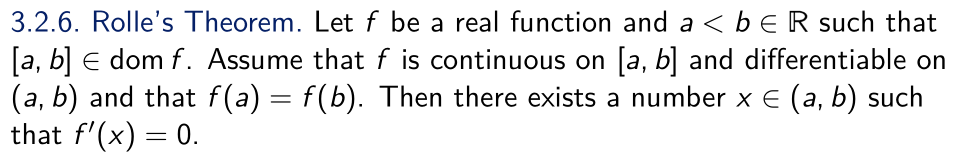
\includegraphics[width=0.9\textwidth]{2020-11-04-12-17-48.png}
    \end{figure}
    \begin{figure}[H]
        \centering
        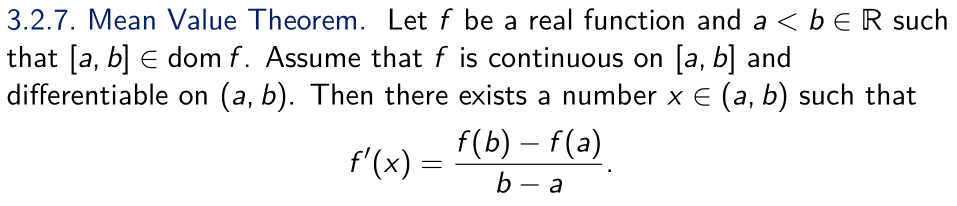
\includegraphics[width=0.9\textwidth]{2020-11-04-12-18-05.png}
    \end{figure}
\end{frame}

\begin{frame}
    \frametitle{Monotonicity}

    \begin{figure}[H]
        \centering
        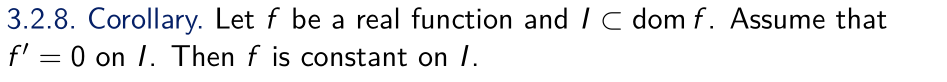
\includegraphics[width=0.9\textwidth]{2020-11-04-12-31-05.png}
    \end{figure}
    \begin{figure}[H]
        \centering
        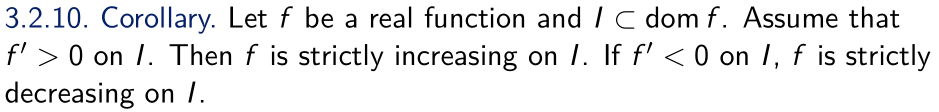
\includegraphics[width=0.9\textwidth]{2020-11-04-12-31-21.png}
    \end{figure}
\end{frame}


\begin{frame}
    \frametitle{Maxima and Minima}
    Here come two important theorems which are easily confused.
    \begin{figure}[H]
        \centering
        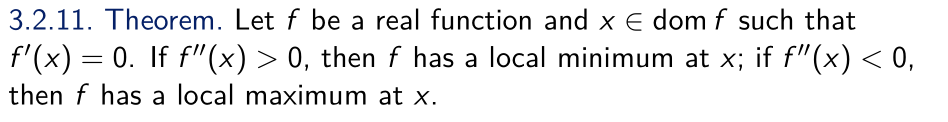
\includegraphics[width=0.9\textwidth]{2020-11-04-12-36-35.png}
    \end{figure}
    \begin{figure}[H]
        \centering
        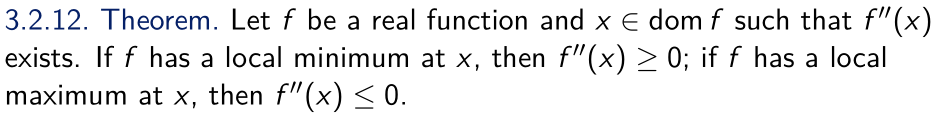
\includegraphics[width=0.9\textwidth]{2020-11-04-12-36-50.png}
    \end{figure}
\end{frame}

\subsection{Convexity and Concavity}
\begin{frame}[allowframebreaks]
    \frametitle{Convexity and Concavity}
    \begin{figure}[H]
        \centering
        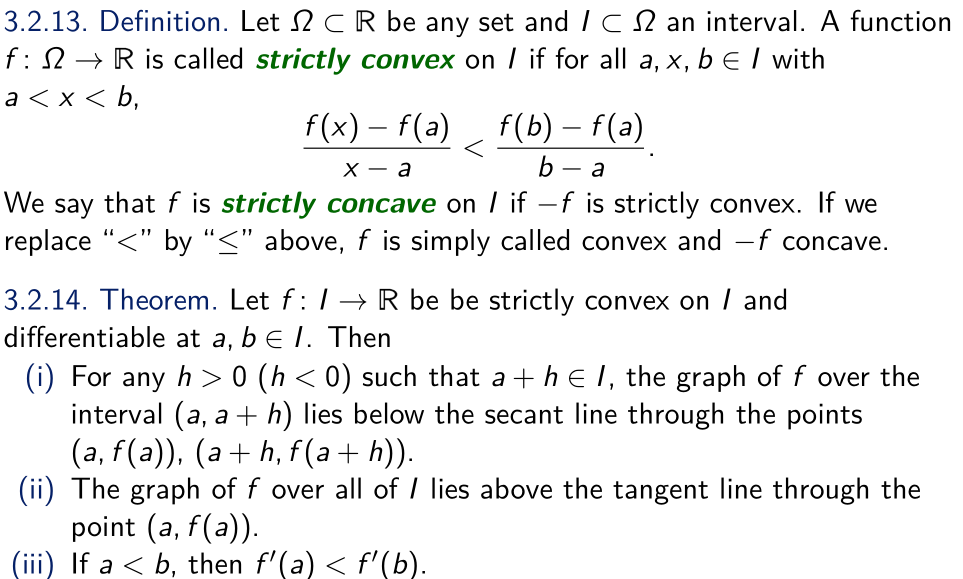
\includegraphics[width=0.9\textwidth]{2020-11-04-12-39-22.png}
    \end{figure}
    \begin{figure}[H]
        \centering
        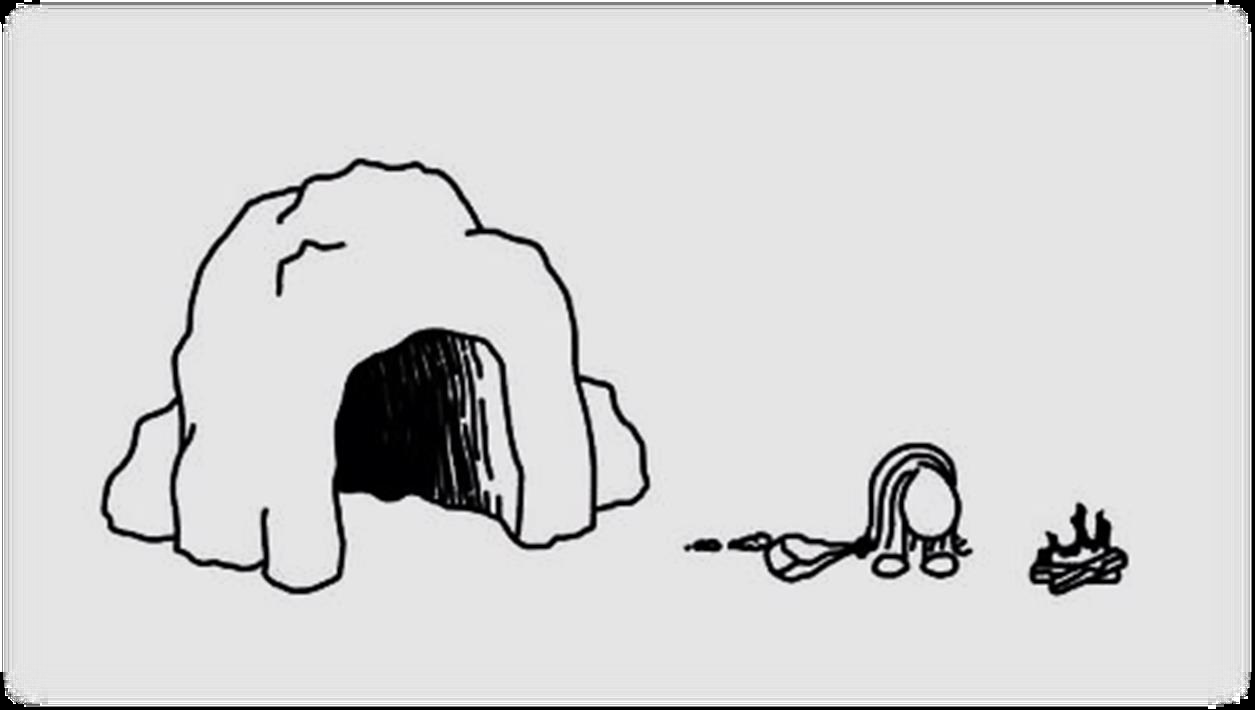
\includegraphics[width=0.6\textwidth]{2020-11-04-17-15-27.png}
        \caption{Concave}
    \end{figure}

\end{frame}

\subsection{\textbf{Curve Sketching}}
\begin{frame}
    \frametitle{\textbf{Curve Sketching}}
    \begin{itemize}
        \item
              $99\%$ possibility to appear in your midterm 2.
        \item Follow the guidelines provided by Horst. (The rubric will be generally the same as the guidelines.)\footnote[frame]{Please refer to Slides 312!!!}
    \end{itemize}
    \begin{figure}[H]
        \centering
        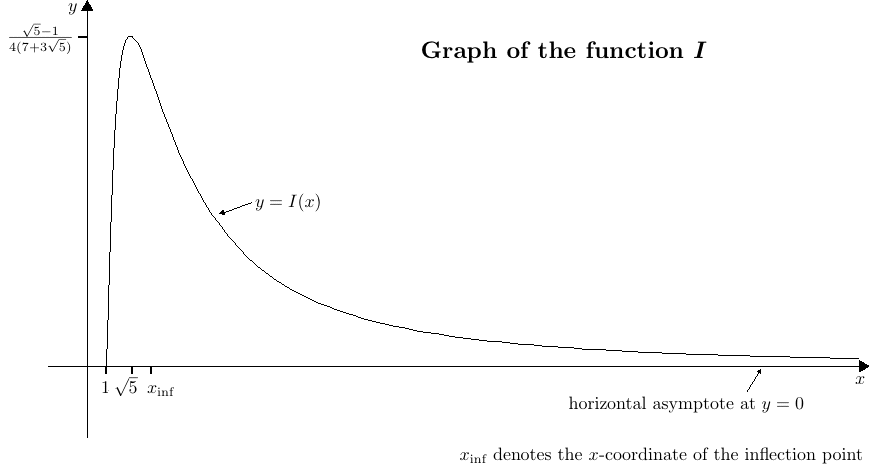
\includegraphics[width=0.5\textwidth]{2020-11-04-12-46-58.png}
    \end{figure}
    Two advice:
    \begin{enumerate}
        \item Do not forget to mark the \emph{asymptote line}.
        \item Do not add any \textbf{redundant} marks.
    \end{enumerate}
\end{frame}

\begin{frame}
    \frametitle{Exercise}

    Consider the function $f: \mathbb{R} \rightarrow \mathbb{R}$ given by
    $$
        f(x)=\frac{x}{1+e^{-x}}
    $$
    \begin{enumerate}
        \item
              Find all local and global maxima and minima if they exist or explain why they don't exist.
        \item
              Where is $f$ increasing/decreasing?
        \item
              Where is $f$ convex / concave?
        \item
              Find all asymptotes of $f$.
        \item
              Sketch the graph of $f,$ indicating any asymptotes and marking characteristic points on the axes.
    \end{enumerate}


\end{frame}

\subsection{L’Hôpital’s Rule}
\begin{frame}
    \frametitle{L’Hôpital’s Rule}
    $$\underset{x\searrow b}{\lim}\dfrac{f(x)}{g(x)}=\underset{x\searrow b}{\lim}\dfrac{f'(x)}{g'(x)}$$
    if$\underset{x\searrow b}{\lim}f(x)=\underset{x\searrow b}{\lim}g(x)=0 \text{ or }\infty$, and $\underset{x\searrow b}{\lim}\dfrac{f'(x)}{g'(x)}$ exists.
    \nullspace
    \textbf{Question: }\\
    Find limit of $$f(x)=\frac{\sqrt{x+3}-\sqrt{3 x+1}}{x-1}$$ at $x=1$.
\end{frame}

\section{Vector Space}
\subsection{Vector Space}
\begin{frame}[allowframebreaks]
    \frametitle{Vector Space}
    \emph{Vector space} is definitely \textbf{the most important algebraic structure} in Honors Mathematics. We will exploit many nice properties and useful application of it throughout VV186 to VV286.
    \nullspace
    Thus, for now, let's remember its definition firmly.
    \begin{figure}[H]
        \centering
        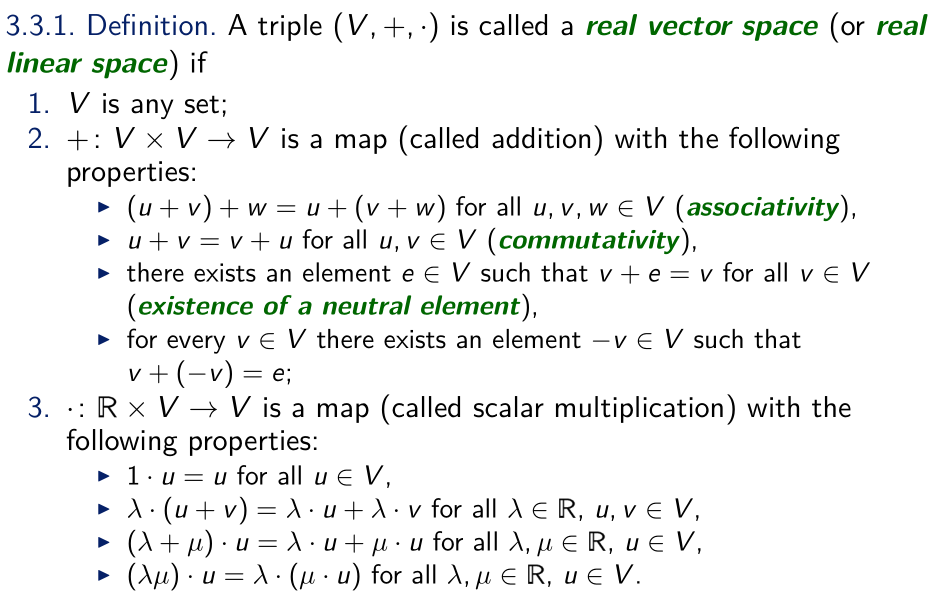
\includegraphics[width=0.9\textwidth]{2020-11-04-15-49-39.png}
    \end{figure}
    What is a \emph{complex vector space}? What is the difference between real and complex vector spaces in definition?\nullspace
    Here is a list of examples:
    \begin{enumerate}
        \item $\R^n$
        \item $\mathbb{C}^n$
        \item $C(\Omega)$
        \item $C^k(\Omega)$
        \item $C^\infty(\Omega)$
        \item $\ell^p:=\{(x_n):\sum_{n}\left|x_{n}\right|^{p}<\infty\}$
        \item $\mathcal{L}(U,V)$: The set of all linear maps from $U$ to $V$, where $U,V$ are both vector space.
        \item* $\mathcal{L}(U,\mathcal{L}(U,V))$
        \item $\operatorname{Mat}(m\times n;\R)$: The set of all $m$-by-$n$ matrices.
    \end{enumerate}
\end{frame}

\begin{frame}
    \frametitle{Subspace}
    A vector space may contain a smaller vector space.
    \begin{figure}[H]
        \centering
        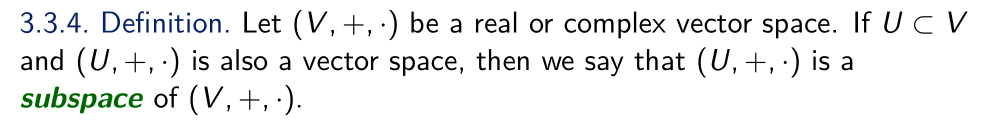
\includegraphics[width=0.9\textwidth]{2020-11-04-16-08-33.png}
    \end{figure}
    It turns out that we do not bother to prove all 9 properties of $(U,+,\cdot)$ to deduce it is also a vector space:
    \begin{figure}[H]
        \centering
        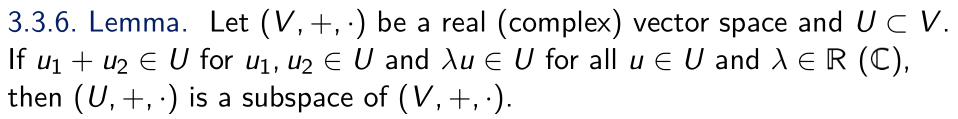
\includegraphics[width=0.9\textwidth]{2020-11-04-16-10-47.png}
    \end{figure}
    \textbf{Remark:} Every vector space has at least one subspace which contains only its zero element. i.e. $(\{0\},+,\cdot)$. We call this space the \emph{trivial space}.
\end{frame}

\begin{frame}
    \frametitle{True of False?}

     A real vector space is a subspace of $\R^n$, a complex vector space is a subset of $\mathbb{C}^n$.
    \nullspace
     \pause False. Real/Complex describes how can we perform scalar multiplication.
\end{frame}

\subsection{Normed Vector Space}
\begin{frame}
    \frametitle{Normed Vector Space}

    With a nice math structure, we still want even more. We want to define a \textit{measure of length} for every element in the vector space.
    \pause
    \begin{figure}[H]
        \centering
        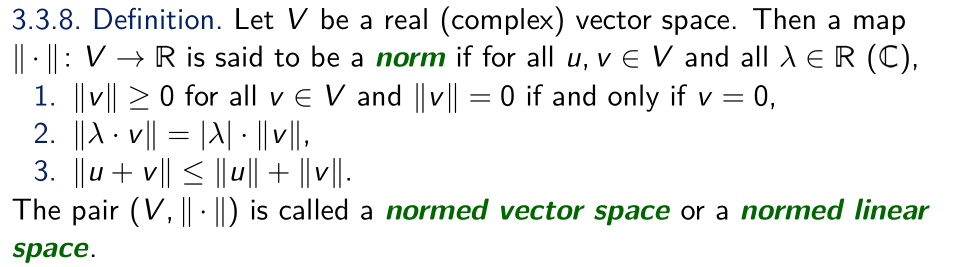
\includegraphics[width=0.9\textwidth]{2020-11-04-16-17-22.png}
    \end{figure}
    \textbf{Remark:}
    \begin{itemize}
        \item A normed vector space can be considered as a metric space.
        \item What's the difference between a metric space and a normed vector space?
    \end{itemize}
\end{frame}

\begin{frame}
    \frametitle{True of False?}

    \begin{enumerate}
        \item 
        Given a vector space $V,$ and its two non-empty subspaces $V_{1}, V_{2},$ then $V_{1} \cup V_{2}$ is a subspace of $V$
        \item
        Given a vector space $V,$ and its two subspaces $V_{1}, V_{2},$ then $V_{1} \cap V_{2}$ is a subspace of $V$
        \item
        The set of all linear maps on $\mathbb{R}$ is a subspace of $\mathrm{C}(\mathbb{R})$
        \item
        Given a vector space $\mathbb{R}^{n},$ for any two distinct norms $\|\cdot\|_{1},\|\cdot\|_{2}$ of $\mathbb{R}^{n},\|\cdot\|:=$ $\sqrt{\|\cdot\|_{1}\|\cdot\|_{2}}$ is also a norm of $\mathbb{R}^{n}$
        \item
        Given a vector space $V,$ given two norms $\|\cdot\|_{1}: V \rightarrow \mathbb{R} ;\|\cdot\|_{2}: \mathbb{R} \rightarrow \mathbb{R},$ then the $\|\cdot\|:=\|\cdot\|_{2} \circ\|\cdot\|_{1}$ is a norm of $V$
    \end{enumerate}

\end{frame}

\begin{frame}
    \frametitle{End}
    \vspace{2.2cm}
    \begin{center}
        \Large
        Have Fun \\
        And \\
        Learn Well!\footnote[frame]{Special acknowledgement to former TA \textbf{Zhang Leyang}, who offered plenty of exercises and advice to my recitation class.}
    \end{center}
\end{frame}

\end{document}